Ant Colony Optimization (ACO) is a \textit{metaheuristic} algorithm inspired by the behavior of real ants, particularly their foraging behavior, which involves depositing pheromones to guide other ants toward food sources. A metaheuristic refers to a higher-level procedure designed to find, generate, or select a heuristic that can provide good solutions to complex optimization problems, often by exploring a large solution space in a way that is not guaranteed to be optimal, but likely to be good enough in a reasonable time frame. This nature-inspired algorithm, introduced by Marco Dorigo in the early 1990s, has been successfully applied to a variety of NP-hard and NP-complete problems, such as the Traveling Salesman Problem (TSP), vehicle routing, and network optimization \cite{Dorigo2004}. One particularly challenging NP-hard problem is the Maximum Matching Problem which is essential in fields like network design, job assignments, and resource allocation.

This book explores how ACO can be adapted to solve the Maximum Matching Problem. The sections following describe how ACO works,its adaptation for solving the Maximum Matching Problem, and its application in other NP-hard problems.

\subsubsection*{Background on Ant Colony Optimization}

Ant Colony Optimization (ACO) mimics the way real ants use pheromones to communicate and find optimal paths between their nest and a food source. As illustrated in figure ~\ref{fig:ant_pheromone_path}, the diagram demonstrates this behavior in a simplified form. The nest (represented by the yellow circle) is located at the origin, while the food source (red circle) is positioned at a distance. Ants travel along different paths, each marked by different colors which represent different pheromone trails. In the diagram, the \textbf{high pheromone trail} (blue line) represents the optimal path, where ants have reinforced the trail most frequently. The \textbf{medium pheromone trail} (black line) and \textbf{low pheromone trail} (red line) represent paths that have seen less traffic and, therefore, lower pheromone concentrations.
 

\begin{figure}[t]
\centering
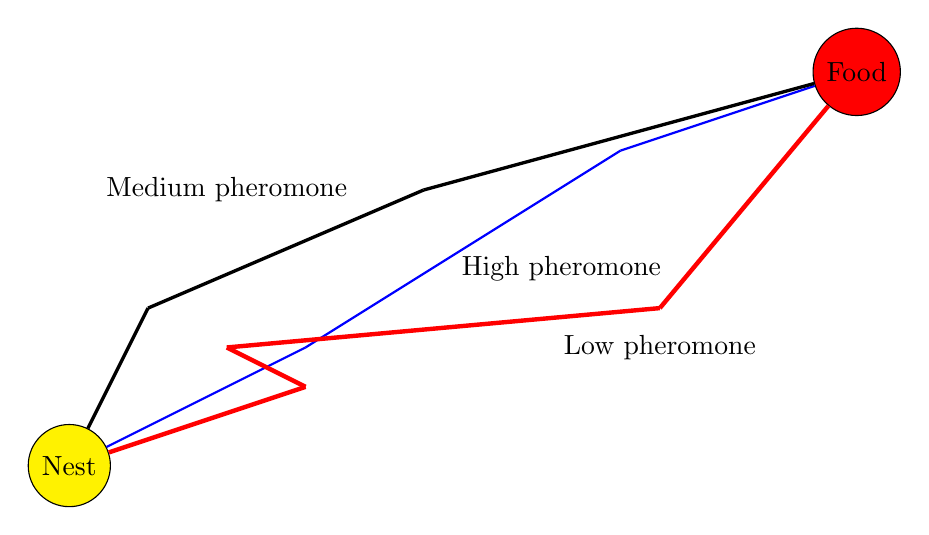
\begin{tikzpicture}
    % Define nodes for nest and food source
    \node[draw, circle, fill=yellow] (nest) at (0, 0) {Nest};
    \node[draw, circle, fill=red] (food) at (10, 5) {Food};

    % Ant paths with varying pheromone strengths (represented by line thickness)
    \draw[thick, color=blue] (nest) -- (3, 1.5);
    \draw[thick, color=blue] (3, 1.5) -- (7, 4);
    \draw[thick, color=blue] (7, 4) -- (food);

    \draw[very thick] (nest) -- (1, 2);
    \draw[very thick] (1, 2) -- (4.5, 3.5);
    \draw[very thick] (4.5, 3.5) -- (food);

    \draw[ultra thick, color=red] (nest) -- (3, 1);
    \draw[ultra thick, color=red] (3, 1) -- (2, 1.5);
    \draw[ultra thick, color=red] (2, 1.5) -- (7.5, 2);
    \draw[ultra thick, color=red] (7.5, 2) -- (food);

    % Labels for pheromone intensity
    \node at (7.5, 1.5) {Low pheromone};
    \node at (2, 3.5) {Medium pheromone};
    \node at (6.25, 2.5) {High pheromone};
\end{tikzpicture}
\caption{A diagram illustrating how ants use pheromones to find the optimal path from the nest to a food source.}
\label{fig:ant_pheromone_path}
\end{figure}


Similarly, Artificial ants in ACO build solutions incrementally, influenced by pheromone trails that are reinforced by previously discovered good solutions.

ACO operates in iterations where each ant constructs a solution using a probabilistic rule based on the amount of pheromone and problem-specific heuristic information\cite{Dorigo2004}. After the construction phase, pheromones are updated based on the quality of the solutions generated, allowing future ants to exploit these trails. Over time, good solutions receive more pheromone reinforcement, while poorer paths evaporate, preventing the over-exploration of suboptimal areas.

ACO was initially applied to the Traveling Salesman Problem, a classic NP-hard problem where the goal is to find the shortest possible route that visits a set of cities and returns to the origin. Marco Dorigo demonstrated that ACO’s flexible framework and ability to find near-optimal solutions in complex search spaces made it well-suited for TSP and similar problems, including vehicle routing and job-shop scheduling \cite{Stutzle2011}.
\newpage

\subsubsection*{Adapting ACO for Maximum Matching}

While Ant Colony Optimization (ACO) has been widely applied to various combinatorial optimization problems, its application to the Maximum Matching Problem is relatively recent. The main challenge in adapting ACO for this problem is modifying the pheromone update mechanism to handle the constraints inherent in matching within graphs, where each vertex can only be part of a single matching edge. 

First, let \( G = (V, E) \) represent an undirected graph, where \( V \) is the set of vertices and \( E \) is the set of edges. We assume the graph is bipartite, meaning the vertices are divided into two disjoint sets \( V_1 \) and \( V_2 \), with edges only connecting vertices from \( V_1 \) to \( V_2 \).

Each edge \( (u, v) \in E \) is assigned a pheromone level \( \tau_{uv} \), initialized to a small constant value \( \tau_0 \). In addition, we define a heuristic function \( \eta_{uv} \), which could represent the inverse of the edge weight, or in the case of an unweighted graph, a constant value.

\[
\tau_{uv} \leftarrow \tau_0, \quad \forall (u, v) \in E
\]

Each ant begins at a vertex and constructs a matching by selecting edges probabilistically, based on the pheromone levels and heuristic values. The probability \( P_{uv} \) of selecting an edge \( (u, v) \) is given by the following formula:

\[
P_{uv} = \frac{\tau_{uv}^\alpha \eta_{uv}^\beta}{\sum_{(u, w) \in N(u)} \tau_{uw}^\alpha \eta_{uw}^\beta}
\]

where:
\begin{itemize}
    \item \( \tau_{uv} \) is the pheromone level on edge \( (u, v) \),
    \item \( \eta_{uv} \) is the heuristic function associated with edge \( (u, v) \),
    \item \( \alpha \) and \( \beta \) are parameters controlling the relative importance of pheromone and heuristic information,
    \item \( N(u) \) represents the set of neighbors of vertex \( u \).
\end{itemize}

Ants select edges based on these probabilities, with edges containing higher pheromone levels being more likely to be chosen. Once an ant selects an edge \( (u, v) \), it adds the edge to its current matching and moves to the next vertex, continuing until no more valid edges can be selected.

After all ants have constructed their matchings, the pheromones are updated in two stages: evaporation and reinforcement. The pheromone on each edge is updated based on the quality of the solutions found by the ants. If an ant has discovered a good matching, the pheromone on the edges used by that ant is increased. The global pheromone update rule is as follows:

\[
\tau_{uv} \leftarrow (1 - \rho) \tau_{uv} + \rho \Delta \tau_{uv}
\]

where:
\begin{itemize}
    \item \( \rho \) is the evaporation rate, controlling how quickly pheromones decay,
    \item \( \Delta \tau_{uv} \) is the pheromone deposit on edge \( (u, v) \), typically proportional to the quality of the solution.
\end{itemize}

During the solution construction phase, ants also perform a local pheromone update to encourage exploration of different edges. The pheromone on an edge \( (u, v) \) is slightly reduced:

\[
\tau_{uv} \leftarrow (1 - \alpha) \tau_{uv}
\]

where \( \alpha \) is a small constant.

The algorithm continues iterating until a predefined number of iterations, \( T \), is reached or until the pheromone values stabilize, indicating convergence. Once this condition is met, the best solution found is returned as the maximum matching.

This demonstrates the application of Ant Colony Optimization to the Maximum Matching problem. By simulating the foraging behavior of ants and utilizing pheromone updates, ACO is capable of effectively exploring the solution space and finding solutions that approach optimality. While ACO may not always guarantee an optimal solution, it offers a flexible and efficient approach for large, complex graphs where traditional exact algorithms may not be feasible.

To illustrate how ACO works on a bipartite graph, consider figure \ref{fig:ACObipartite_graph}. 

\begin{figure}[t]
    \centering
    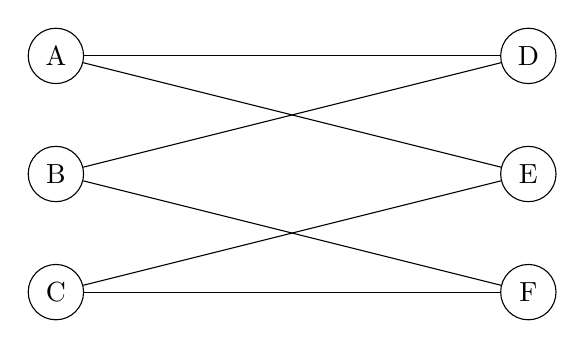
\begin{tikzpicture}[scale=1.5]
    \tikzset{vertex/.style = {shape=circle,draw,minimum size=2em}}
    \tikzset{edge/.style = {-,> = latex'}}
    % vertices on the left
    \node[vertex] (a) at (0,1) {A};
    \node[vertex] (b) at (0,0) {B};
    \node[vertex] (c) at (0,-1) {C};
    % vertices on the right
    \node[vertex] (d) at (4,1) {D};
    \node[vertex] (e) at (4,0) {E};
    \node[vertex] (f) at (4,-1) {F};
    % edges
    \draw (a) to (d);
    \draw (a) to (e);
    \draw (b) to (d);
    \draw (b) to (f);
    \draw (c) to (e);
    \draw (c) to (f);
    \end{tikzpicture}
    \caption{Initial 3x3 bipartite graph for the Maximum Matching Problem.}
    \label{fig:ACObipartite_graph}
\end{figure}

\subsubsection*{Step 1: Initialization}
In the first step, we initialize pheromone levels for all edges. Let’s assume a small initial pheromone value $\tau_0$ for all edges (e.g., $\tau_0 = 1$) as seen in figure \ref{fig:Initialized_graph}.

\begin{figure}[t]
    \centering
    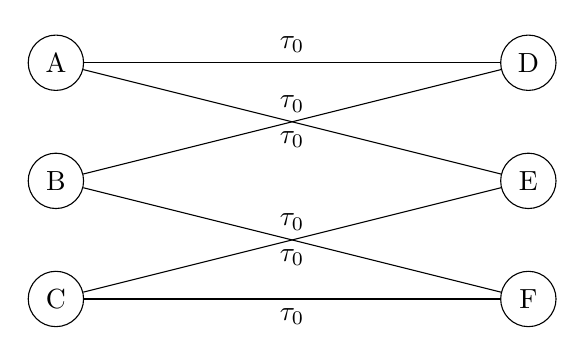
\begin{tikzpicture}[scale=1.5]
    \tikzset{vertex/.style = {shape=circle,draw,minimum size=2em}}
    \tikzset{edge/.style = {-,> = latex'}}
    % vertices on the left
    \node[vertex] (a) at (0,1) {A};
    \node[vertex] (b) at (0,0) {B};
    \node[vertex] (c) at (0,-1) {C};
    % vertices on the right
    \node[vertex] (d) at (4,1) {D};
    \node[vertex] (e) at (4,0) {E};
    \node[vertex] (f) at (4,-1) {F};
    % edges with pheromone values
    \draw (a) to node[midway, above] {$\tau_0$} (d);
    \draw (a) to node[midway, below] {$\tau_0$} (e);
    \draw (b) to node[midway, above] {$\tau_0$} (d);
    \draw (b) to node[midway, below] {$\tau_0$} (f);
    \draw (c) to node[midway, above] {$\tau_0$} (e);
    \draw (c) to node[midway, below] {$\tau_0$} (f);
    \end{tikzpicture}
    \caption{Graph with initialized pheromone values ($\tau_0$) on all edges.}
    \label{fig:Initialized_graph}
\end{figure}

\subsubsection*{Step 2: Ants Build Matchings}
Ants start to traverse the graph, selecting edges probabilistically based on pheromone values and a heuristic (e.g., choosing edges with available unmatched vertices). Each ant attempts to construct a matching.

In figure \ref{fig:Ant_selection} there are three ants, with Ant 1 starting from vertex A, Ant 2 from vertex B, and Ant 3 from vertex C.

\begin{figure}[t]
    \centering
    \begin{subfigure}[b]{0.3\textwidth}
        \centering
        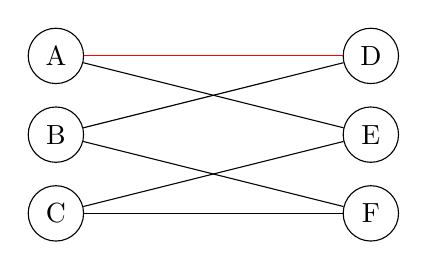
\begin{tikzpicture}
        \tikzset{vertex/.style = {shape=circle,draw,minimum size=2em}}
        \tikzset{edge/.style = {-,> = latex'}}
        % vertices on the left
        \node[vertex] (a) at (0,1) {A};
        \node[vertex] (b) at (0,0) {B};
        \node[vertex] (c) at (0,-1) {C};
        % vertices on the right
        \node[vertex] (d) at (4,1) {D};
        \node[vertex] (e) at (4,0) {E};
        \node[vertex] (f) at (4,-1) {F};
        % edges selected by Ant 1
        \draw[red] (a) to (d);
        \draw (a) to (e);
        \draw (b) to (d);
        \draw (b) to (f);
        \draw (c) to (e);
        \draw (c) to (f);
        \end{tikzpicture}
        \caption{Ant 1 selects edge (A, D).}
    \end{subfigure}
    \begin{subfigure}[b]{0.3\textwidth}
        \centering
        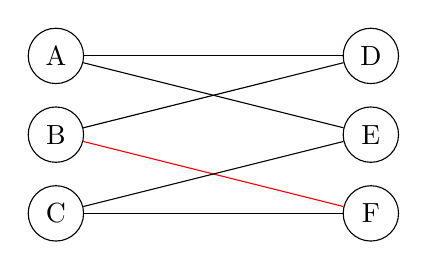
\begin{tikzpicture}
        \tikzset{vertex/.style = {shape=circle,draw,minimum size=2em}}
        \tikzset{edge/.style = {-,> = latex'}}
        % vertices on the left
        \node[vertex] (a) at (0,1) {A};
        \node[vertex] (b) at (0,0) {B};
        \node[vertex] (c) at (0,-1) {C};
        % vertices on the right
        \node[vertex] (d) at (4,1) {D};
        \node[vertex] (e) at (4,0) {E};
        \node[vertex] (f) at (4,-1) {F};
        % edges selected by Ant 2
        \draw (a) to (d);
        \draw (a) to (e);
        \draw[red] (b) to (f);
        \draw (b) to (d);
        \draw (c) to (e);
        \draw (c) to (f);
        \end{tikzpicture}
        \caption{Ant 2 selects edge (B, F).}
    \end{subfigure}
    \begin{subfigure}[b]{0.3\textwidth}
        \centering
        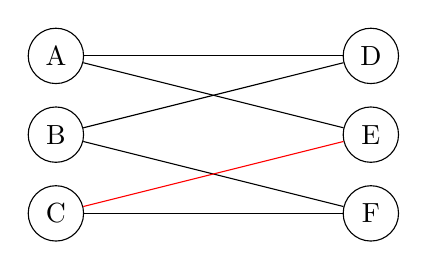
\begin{tikzpicture}
        \tikzset{vertex/.style = {shape=circle,draw,minimum size=2em}}
        \tikzset{edge/.style = {-,> = latex'}}
        % vertices on the left
        \node[vertex] (a) at (0,1) {A};
        \node[vertex] (b) at (0,0) {B};
        \node[vertex] (c) at (0,-1) {C};
        % vertices on the right
        \node[vertex] (d) at (4,1) {D};
        \node[vertex] (e) at (4,0) {E};
        \node[vertex] (f) at (4,-1) {F};
        % edges selected by Ant 3
        \draw (a) to (d);
        \draw (a) to (e);
        \draw (b) to (d);
        \draw (b) to (f);
        \draw[red] (c) to (e);
        \draw (c) to (f);
        \end{tikzpicture}
        \caption{Ant 3 selects edge (C, E).}
    \end{subfigure}
    \caption{Ants constructing matchings by selecting edges probabilistically.}
    \label{fig:Ant_selection}
\end{figure}

\subsubsection*{Step 3: Pheromone Update}
In figure \ref{fig:Pheromone_update} all ants have completed their matchings, and pheromones are updated. Pheromones on the edges selected by the ants are reinforced, while pheromones on other edges evaporate. Let $\Delta\tau$ represent the increase in pheromone for selected edges, and $\epsilon$ represent the evaporation factor.

\begin{figure}[t]
    \centering
    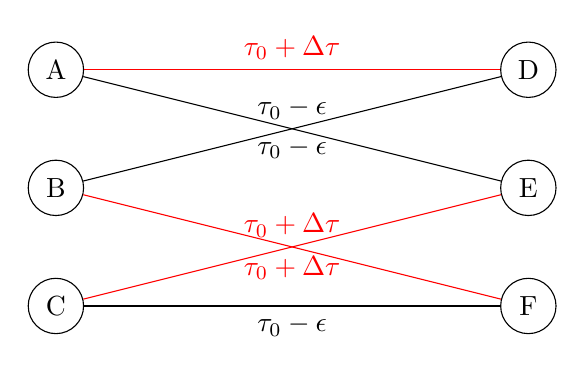
\begin{tikzpicture} [scale=1.5]
    \tikzset{vertex/.style = {shape=circle,draw,minimum size=2em}}
    \tikzset{edge/.style = {-,> = latex'}}
    % vertices on the left
    \node[vertex] (a) at (0,1) {A};
    \node[vertex] (b) at (0,0) {B};
    \node[vertex] (c) at (0,-1) {C};
    % vertices on the right
    \node[vertex] (d) at (4,1) {D};
    \node[vertex] (e) at (4,0) {E};
    \node[vertex] (f) at (4,-1) {F};
    % edges with pheromone updates
    \draw[red] (a) to node[midway, above] {$\tau_0 + \Delta\tau$} (d);
    \draw (a) to node[midway, below] {$\tau_0 - \epsilon$} (e);
    \draw[red] (b) to node[midway, above] {$\tau_0 + \Delta\tau$} (f);
    \draw (b) to node[midway, above] {$\tau_0 - \epsilon$} (d);
    \draw[red] (c) to node[midway, below] {$\tau_0 + \Delta\tau$} (e);
    \draw (c) to node[midway, below] {$\tau_0 - \epsilon$} (f);
    \end{tikzpicture}
    \caption{Pheromone update after constructing valid matchings.}
    \label{fig:Pheromone_update}
\end{figure}

\subsubsection*{Step 4: Repeat the Process (Multiple Iterations)}
The ants will repeat the process for a number of iterations, each time constructing matchings and updating the pheromone levels. The goal is to encourage the ants to explore edges that are part of high-quality matchings, while discouraging exploration of less optimal edges. Over time, the pheromone levels on better edges will accumulate, guiding future ants towards those edges.

For simplicity, let’s assume 3 iterations. After each iteration, pheromone values are updated, and ants select their next edges based on the updated pheromone levels.

\paragraph{Iteration 2 (After Updating Pheromone from Iteration 1):}
The ants will once again probabilistically select edges based on the pheromone levels, with a higher probability for edges that have been chosen frequently in the previous iteration (since they have higher pheromone levels).

In figure \ref{fig:ants2_selection} ant 1 selects a different edge based on the updated pheromone values:

\begin{figure}[t]
\centering
\begin{subfigure}[b]{0.3\textwidth}
\centering
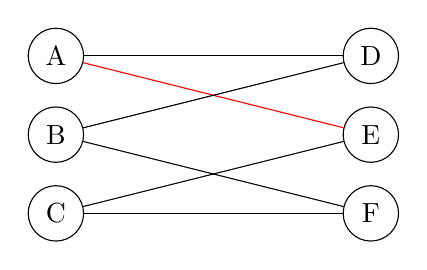
\begin{tikzpicture}
\tikzset{vertex/.style = {shape=circle,draw,minimum size=2em}}
\tikzset{edge/.style = {-,> = latex'}}
% vertices on the left
\node[vertex] (a) at (0,1) {A};
\node[vertex] (b) at (0,0) {B};
\node[vertex] (c) at (0,-1) {C};
% vertices on the right
\node[vertex] (d) at (4,1) {D};
\node[vertex] (e) at (4,0) {E};
\node[vertex] (f) at (4,-1) {F};
% edges selected by Ant 1 after pheromone update
\draw[red] (a) to (e); % Ant 1 switches to (A, E) after pheromone update
\draw (a) to (d);
\draw (b) to (d);
\draw (b) to (f);
\draw (c) to (e);
\draw (c) to (f);
\end{tikzpicture}
\caption{Ant 1 now selects edge (A, E).}
\end{subfigure}
\begin{subfigure}[b]{0.3\textwidth}
\centering
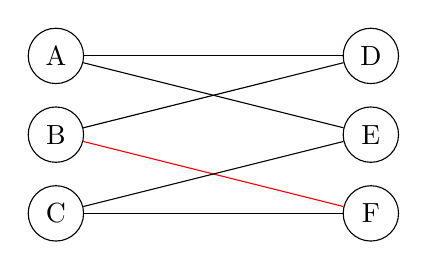
\begin{tikzpicture}
\tikzset{vertex/.style = {shape=circle,draw,minimum size=2em}}
\tikzset{edge/.style = {-,> = latex'}}
% vertices on the left
\node[vertex] (a) at (0,1) {A};
\node[vertex] (b) at (0,0) {B};
\node[vertex] (c) at (0,-1) {C};
% vertices on the right
\node[vertex] (d) at (4,1) {D};
\node[vertex] (e) at (4,0) {E};
\node[vertex] (f) at (4,-1) {F};
% edges selected by Ant 2 after pheromone update
\draw[red] (b) to (f); % Ant 2 sticks with (B, F)
\draw (a) to (d);
\draw (a) to (e);
\draw (b) to (d);
\draw (c) to (e);
\draw (c) to (f);
\end{tikzpicture}
\caption{Ant 2 sticks with edge (B, F).}
\end{subfigure}
\begin{subfigure}[b]{0.3\textwidth}
\centering
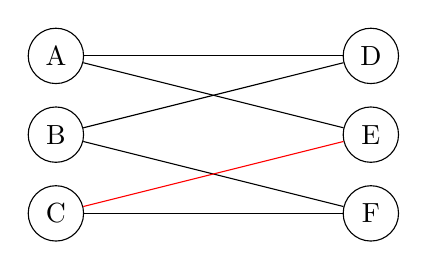
\begin{tikzpicture}
\tikzset{vertex/.style = {shape=circle,draw,minimum size=2em}}
\tikzset{edge/.style = {-,> = latex'}}
% vertices on the left
\node[vertex] (a) at (0,1) {A};
\node[vertex] (b) at (0,0) {B};
\node[vertex] (c) at (0,-1) {C};
% vertices on the right
\node[vertex] (d) at (4,1) {D};
\node[vertex] (e) at (4,0) {E};
\node[vertex] (f) at (4,-1) {F};
% edges selected by Ant 3 after pheromone update
\draw (c) to (f); 
\draw (a) to (d);
\draw (a) to (e);
\draw (b) to (d);
\draw (b) to (f);
\draw[red] (c) to (e);
\end{tikzpicture}
\caption{Ant 3 sticks with edge (C, E).}
\end{subfigure}
\caption{Ants constructing failed matchings after pheromone update.}
\label{fig:ants2_selection}
\end{figure}

\subsubsection*{Step 5: Evaluating and Improving the Matchings}
After several iterations, the ants will converge towards the edges that form the best matching. The pheromone values on these edges will be much higher, guiding future ants toward these edges. At the end of the process, you can evaluate the total matching based on the pheromone values accumulated across iterations.

Let’s assume the following results after 3 iterations:

\begin{itemize}
  \item Ant 1 successfully matched A to D.
  \item Ant 2 matched B to F.
  \item Ant 3 matched C to E.
\end{itemize}

The total matching could be:

\begin{itemize}
  \item A - D
  \item B - F
  \item C - E
\end{itemize}

This is a maximum matching because each vertex on the left is matched with exactly one vertex on the right, and no more matchings can be made without violating the constraints of the bipartite graph.

\subsubsection*{Step 6: Final Pheromone Adjustment and Conclusion}
In the final step, pheromones are updated again, ensuring that the best edges (those contributing to the maximum matching) are reinforced. Ants now have a high probability of selecting these edges in future iterations, and the algorithm converges to the optimal or near-optimal solution.

In this case, the matching A - D, B - F, and C - E is likely the optimal solution, which the algorithm has successfully found after several iterations of pheromone updates and edge selections.

\paragraph{}This example illustrates how the Ant Colony Optimization (ACO) algorithm can be adapted to solve the Maximum Matching Problem in bipartite graphs. The key steps of the process—edge selection based on pheromones, iterative construction of matchings, and pheromone updates—guide the ants toward an optimal solution. Through repeated iterations, the algorithm efficiently converges towards the maximum matching.




\subsubsection*{Ant Colony Optimization for NP Problems}
Ant Colony Optimization (ACO) has been widely applied to NP-hard problems due to its ability to find approximate solutions in complex search spaces. Among these problems, subset problems—where the goal is to find a subset of items that maximizes or minimizes a certain objective—are particularly significant. This section explores how ACO has been adapted for four well-known subset problems: the Traveling Salesman Problem (TSP), the Knapsack Problem, the Set Covering Problem, and the Independent Set Problem.

\paragraph{Traveling Salesman Problem (TSP):}
The Traveling Salesman Problem (TSP) is one of the most extensively studied NP-hard problems in combinatorial optimization. It requires finding the shortest possible route that visits a given set of cities exactly once and returns to the starting point. TSP is central in various fields, including logistics, routing, and manufacturing, where minimizing travel costs or time is essential. Despite its simple formulation, the computational complexity of TSP arises from the exponential growth in possible routes as the number of cities increases, making it impractical to solve through brute force methods for larger instances.

Ant Colony Optimization (ACO) was first successfully applied to the TSP by Dorigo et al. \cite{Dorigo2004}. Each ant in this system represents a potential solution, or route, and the algorithm mimics how real ants use pheromone trails to mark favorable paths. In the ACO for TSP, pheromones guide the selection of cities to visit, with shorter, more optimal routes receiving stronger pheromone reinforcement. This process of iterative pheromone updates allows the algorithm to increasingly favor better routes over time. Notably, the method was effective in discovering near-optimal solutions, particularly in cases where traditional heuristics like the nearest-neighbor approach were less efficient.

Later work by Leguizamon and Michalewicz \cite{Leguizamon1999} extended ACO's application to TSP by proposing a new version of the ant system specifically tailored to handle larger problem instances. Their approach emphasized balancing the exploration of new routes with the exploitation of known good solutions, a critical factor in ensuring that the algorithm did not prematurely converge on suboptimal routes. By introducing new mechanisms to control pheromone decay and deposit rates, their version of the ant system was able to maintain diversity in the search space while ensuring that promising routes were reinforced.

In evaluating the effectiveness of ACO on the TSP, both Dorigo and Leguizamon used benchmark datasets such as the TSPLIB to assess solution quality and computational efficiency. Metrics like the average tour length, computational time, and convergence rate were compared against established heuristics, such as the nearest-neighbor and genetic algorithms. In multiple cases, ACO demonstrated superior performance, particularly in terms of finding shorter routes and exhibiting robustness on larger, more complex instances of TSP. The ability to balance exploration and exploitation allowed ACO to outperform traditional approaches under certain conditions, especially as the problem size increased \cite{Stutzle2011}.

The adaptive nature of ACO made it particularly effective in solving TSP. By adjusting the algorithm’s parameters—such as the rate of pheromone evaporation and the amount of pheromone deposited—researchers could fine-tune the balance between intensification (exploiting known good routes) and diversification (exploring new ones). This flexibility enabled ACO to scale effectively and tackle larger instances of the problem, where other methods typically failed or required excessive computational resources.


\paragraph{Knapsack Problem:}
The Knapsack Problem is a classic NP-complete combinatorial optimization problem where the objective is to choose a subset of items, each with a specific weight and value, such that the total value is maximized without exceeding the weight capacity of a knapsack. This problem is central in fields like resource allocation, budgeting, and decision-making where a trade-off between constraints (e.g., weight) and rewards (e.g., value) needs to be balanced. Due to its computational complexity, exact algorithms often become impractical for large instances, making heuristic approaches like Ant Colony Optimization (ACO) an appealing alternative.

ACO can be adapted to solve the Knapsack Problem by viewing item selection as a path-building process, where each ant represents a candidate solution (a subset of items). In this context, the pheromone trails are used to guide the selection of items based on their value-to-weight ratio. As ants explore various item combinations, they reinforce those combinations that lead to higher total values without exceeding the knapsack's capacity. Pheromone updates play a crucial role in this iterative process, encouraging future ants to choose item combinations that have been proven successful by earlier ants.

Thomas Stützle describes how ACO can be applied to the Knapsack Problem by incorporating pheromone updates based on the quality of the solutions\cite{Stutzle2011}. In this approach, ants explore different subsets of items, and those that produce higher values within the given capacity constraints are reinforced. This reinforcement leads to a more informed search in future iterations, progressively guiding the ants towards optimal or near-optimal solutions. The algorithm’s adaptive nature allows it to dynamically adjust its search strategy based on the performance of past solutions, making it well-suited for tackling the inherent complexity of the Knapsack Problem.

In addition to the basic ACO framework, hybrid approaches have been developed to further improve solution quality for the Knapsack Problem. For instance, combining ACO with local search techniques, such as dynamic programming or greedy algorithms, enhances the algorithm's performance, particularly when dealing with large item sets or complex constraints. These hybrid methods allow ACO to refine its solutions by exploiting the strengths of local search to intensify the search in promising areas of the solution space, while maintaining ACO's exploratory capabilities. This combination often leads to better results than using ACO or traditional methods in isolation, especially in complex, large-scale instances \cite{Stutzle2011}.

Evaluations of ACO's effectiveness on the Knapsack Problem are typically conducted using benchmark instances. Key performance metrics include solution quality (the total value of selected items), computational efficiency, and the ability to scale to larger problem instances. Comparative studies have demonstrated that ACO, especially when hybridized with local search techniques, can outperform traditional methods in terms of finding high-quality solutions within reasonable computational timeframes, particularly when exact algorithms become infeasible for larger datasets.

\paragraph{Set Covering Problem (SCP)}
The Set Covering Problem (SCP) is a classic NP-complete problem that requires finding the smallest subset of sets whose union covers all elements in a given universal set. SCP appears in a wide variety of practical applications, such as resource allocation, network design, facility location, and scheduling. The challenge with SCP is its combinatorial explosion: as the number of sets grows, the number of possible combinations increases exponentially. This makes exact solutions computationally expensive, particularly for large-scale instances.

Ant Colony Optimization (ACO) is an effective method for tackling SCP, as it excels in exploring large solution spaces and can dynamically adapt to the problem’s constraints. In ACO's application to SCP, each ant incrementally builds a solution by selecting sets to include, aiming to cover all elements in the universal set. Pheromones deposited on sets guide the ants in future iterations, encouraging the selection of sets that have historically been part of good solutions.

Ankit Pat enhanced the ACO algorithm for SCP by adapting the pheromone update mechanism\cite{Pat2014}. In this variant, ants are rewarded for selecting sets that either cover more elements or contribute to smaller overall solutions. The pheromone levels are adjusted after each iteration to reflect the quality of the solution, favoring sets that help achieve a complete cover with minimal redundancy. This approach allows the algorithm to focus on sets that are frequently part of optimal or near-optimal solutions, gradually improving the quality of the solution with each cycle \cite{Pat2014}.

The primary computational difficulty in SCP lies in evaluating all possible combinations of sets, especially as the problem size increases. Traditional approaches, such as greedy algorithms, attempt to build solutions quickly but often result in suboptimal results due to their myopic nature. Exact methods, such as branch-and-bound or integer programming, provide optimal solutions but become computationally prohibitive for large instances.

ACO addresses this by balancing exploration and exploitation through the use of pheromone trails and heuristic information. Ants explore a wide range of solutions by probabilistically selecting sets based on their pheromone levels and the heuristic value (e.g., how many uncovered elements a set includes). This enables ACO to effectively navigate large solution spaces and avoid local optima.

The effectiveness of ACO in solving SCP has been evaluated on standard benchmark instances, comparing it to both greedy heuristics and exact algorithms. Studies, including those by Marco Dorigo and Ankit Pat, have shown that ACO is highly competitive, particularly on large-scale problems where exact methods are impractical due to time constraints\cite{Pat2014,Dorigo2004}. For example, on datasets with hundreds of sets and elements, ACO was able to find near-optimal solutions in a fraction of the time required by exact methods.

Guillermo Leguizamon and Zbigniew Michalewicz demonstrated that their ACO variant for SCP consistently produced better solutions than traditional heuristic methods\cite{Leguizamon1999}. The results indicated that ACO outperformed the greedy algorithm by finding smaller set covers, especially in instances where the greedy approach failed to adequately balance the coverage of elements with the size of the solution \cite{Leguizamon1999}.

The evaluation metrics typically focus on the size of the solution (i.e., the number of sets selected) and the computational time. ACO has been shown to provide a good balance between solution quality and computational efficiency, making it a viable option for large SCP instances where exact methods are infeasible.

\paragraph{Independent Set Problem (ISP)}
The Independent Set Problem (ISP) is an NP-hard problem where the objective is to find the largest subset of vertices in a graph such that no two vertices in the subset are adjacent. ISP has significant applications in fields like network theory, resource allocation, and scheduling, where minimizing conflicts or dependencies between resources is critical. The complexity of ISP stems from the difficulty of ensuring that no adjacent vertices are included in the independent set, especially in large and dense graphs.

ACO has been adapted to solve ISP by treating the problem as one of selecting a subset of non-adjacent vertices. Each ant explores the graph by adding vertices to its candidate solution while ensuring that the adjacency constraints are respected. Pheromone trails are laid on vertices that lead to larger independent sets, guiding future ants toward promising areas of the solution space.

The challenge in ISP is evaluating the potential inclusion of vertices in a way that respects the adjacency constraints while attempting to maximize the size of the independent set. Greedy algorithms tend to struggle with this problem because they often make short-sighted decisions that lead to suboptimal solutions. Exact methods, such as dynamic programming or backtracking, guarantee optimal solutions but are computationally expensive and impractical for large graphs.

ACO’s approach to ISP involves constructing solutions iteratively, with ants making probabilistic decisions based on pheromone levels and heuristic information. The heuristic typically estimates the benefit of including a vertex, considering both the size of the current independent set and the adjacency constraints. As ants traverse the graph, they reinforce the selection of vertices that have been part of larger independent sets in previous iterations.

The performance of ACO in solving ISP has been evaluated in comparison with both greedy algorithms and exact methods. ACO tends to outperform greedy algorithms, particularly on larger graphs where the problem's complexity increases. Ankit Pat and Thomas Stützle showed that ACO could find significantly larger independent sets than traditional algorithms, especially in dense graphs where the adjacency constraints are more restrictive \cite{Pat2014,Stutzle2011}.

In terms of solution quality, ACO is competitive with exact methods but requires significantly less computational time. For instance, Ankit Pat applied ACO to a variety of graph instances, demonstrating that the algorithm consistently found near-optimal solutions\cite{Pat2014}. The size of the independent set discovered by ACO was often close to the best-known solutions, and in some cases, ACO even matched the performance of exact methods, but with much greater efficiency.

Additionally, hybrid ACO algorithms that incorporate local search techniques have been shown to further enhance the performance of ACO in solving ISP. By refining solutions through small modifications, such as adding or removing a vertex, hybrid approaches can explore a wider range of potential solutions, leading to even larger independent sets in complex graph instances. Hung-Pin Shih highlighted that these hybrid techniques are especially effective when dealing with weighted versions of ISP, where the goal is to maximize the total weight of the selected vertices, not just the size of the set \cite{Shih2008}.

\paragraph{Subset Problems in Other Domains}
Beyond the traditional NP-hard problems, Ant Colony Optimization (ACO) has been successfully applied to a wide range of subset problems across various domains. These applications demonstrate the adaptability and versatility of ACO in tackling diverse optimization challenges by customizing its pheromone update rules and heuristic strategies according to the specific characteristics of each domain.

In network design, ACO has been used to optimize the selection of links in communication networks. The objective is to select a subset of links that minimizes the cost while maintaining connectivity across the network. ACO's flexibility allows it to explore different configurations of network links, and its pheromone update mechanism guides the algorithm towards selecting those links that lead to more efficient and cost-effective network structures. This ability to handle dynamic and complex networks makes ACO an appealing approach for real-world network design problems, especially those involving large and complex network topologies \cite{Dorigo2004}.

In bioinformatics, ACO has been applied to subset selection problems such as selecting genes or proteins relevant to certain biological processes or diseases. The challenge here is to identify the most informative subset of features (such as genes) from a larger set that contribute to accurate predictions or classifications. ACO adapts to bioinformatics problems by using pheromone updates based on the relevance of genes or proteins in the context of a given biological dataset. By doing so, the algorithm can efficiently identify subsets of genes or proteins that maximize predictive accuracy or classification performance, while avoiding overfitting or computational inefficiency \cite{Stutzle2011}.

These diverse applications underscore the broad utility of ACO in solving subset problems across different fields. The ability to dynamically adjust pheromone updates, combined with tailored heuristic strategies for each specific problem, allows ACO to find high-quality solutions in domains as varied as network design and bioinformatics. This adaptability has made ACO a powerful tool for tackling complex subset problems where traditional methods might struggle or fail to provide satisfactory results \cite{Leguizamon1999}.



\paragraph{}In each of these applications, the fundamental mechanism of ACO—building solutions incrementally while reinforcing high-quality components—proves highly effective for subset problems, which often involve large solution spaces and complex constraints.

\subsubsection*{Results and Performance Comparison}
Through extensive research, we have found that Ant Colony Optimization (ACO) has shown significant efficiency in solving various NP-hard problems, such as the Traveling Salesman Problem (TSP), Job Scheduling, and Graph Coloring. These problems, like Maximum Matching, involve large solution spaces and complex optimization criteria, making them difficult to solve efficiently with traditional methods. The adaptability of ACO in these contexts suggests that it could similarly offer an efficient approach to the Maximum Matching problem, particularly in larger and more complex graphs.

The strength of ACO lies in its ability to explore and exploit the search space in a way that balances the trade-off between finding new, potentially better solutions (exploration) and refining known solutions (exploitation). This dynamic nature of the algorithm, combined with its distributed, population-based approach, enables it to handle complex combinatorial optimization problems effectively, even when the solution space grows exponentially. The ability to adaptively update pheromones allows ACO to avoid getting trapped in local minima, a common issue with many traditional optimization methods.

Given these successes in other NP-hard problems, we believe ACO holds strong potential for addressing the Maximum Matching problem. The next logical step in our work is to implement the ACO algorithm, not only for bipartite graphs but also for more graph structures, including d-partite and general graphs. By extending ACO to these broader contexts, we can evaluate its scalability and effectiveness in even more complex matching scenarios. the aim to explore how the algorithm can be tailored to account for the additional complexity introduced by multi-partite and non-bipartite structures. This would involve refining the pheromone update mechanism and ensuring that the algorithm can efficiently handle the diverse constraints and relationships within such graphs. By doing so, we hope to extend the applicability of ACO to a wider range of combinatorial optimization problems, further demonstrating its potential as an efficient solution method for large-scale, complex matching problems.


\subsubsection*{Conclusion}
In conclusion, ACO presents a promising approach to solving the Maximum Matching Problem in bipartite graphs, particularly when scalability is a concern. By adapting the pheromone update rules and integrating local search techniques, ACO can offer a competitive alternative to exact methods for large instances.


